\documentclass[dvipdfmx]{standalone}

\usepackage{gnuplot-lua-tikz}
\usepackage{tikz}

\begin{document}
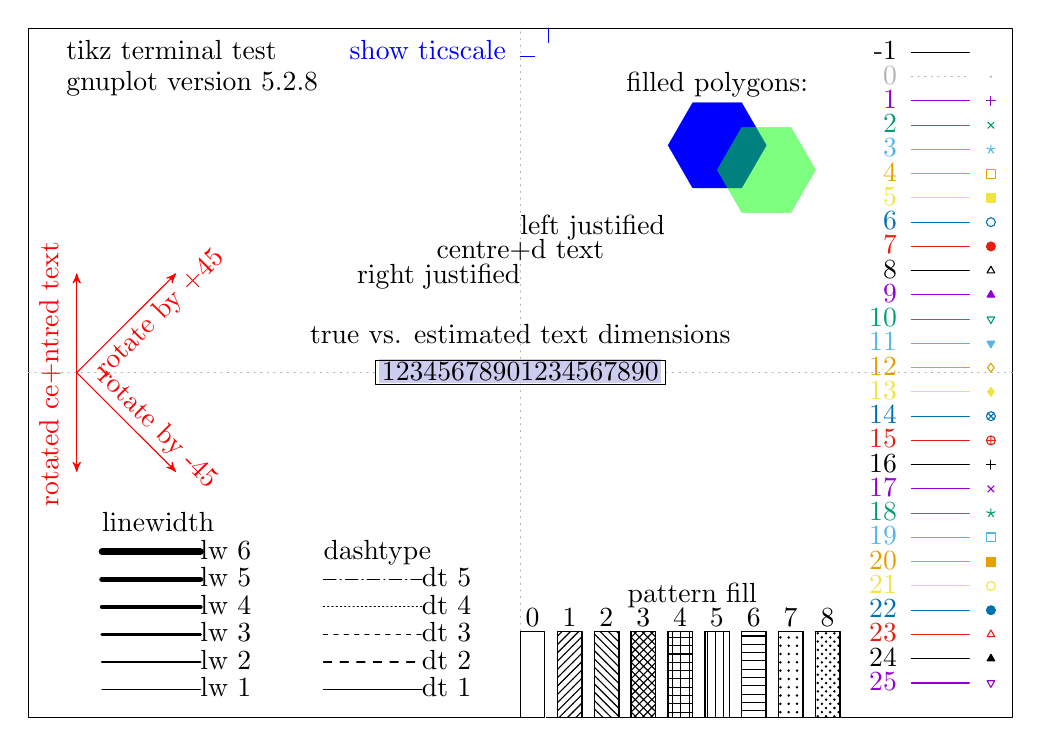
\begin{tikzpicture}[gnuplot]
%% generated with GNUPLOT 5.2p8 (Lua 5.3; terminal rev. Nov 2018, script rev. 108)
%% 2021年05月11日 01時19分42秒
\path (0.000,0.000) rectangle (12.500,8.750);
\gpcolor{color=gp lt color border}
\gpsetlinetype{gp lt border}
\gpsetdashtype{gp dt solid}
\gpsetlinewidth{1.00}
\draw[gp path] (0.000,0.000)--(12.499,0.000)--(12.499,8.749)--(0.000,8.749)--cycle;
\node[gp node left] at (0.368,8.442) {tikz  terminal test};
\node[gp node left] at (0.368,8.057) {gnuplot version 5.2.8  };
\gpcolor{color=gp lt color axes}
\gpsetlinetype{gp lt axes}
\gpsetdashtype{gp dt axes}
\draw[gp path] (6.250,0.000)--(6.250,8.749);
\draw[gp path] (0.000,4.375)--(12.499,4.375);
\gpcolor{color=gp lt color border}
\node[gp node center,inner sep=0pt](gp boxed node 1) at (6.250,4.375) {12345678901234567890};
\gpcolor{rgb color={0.800,0.800,0.933}}
\gpsetlinetype{gp lt border}
\gpsetdashtype{gp dt solid}
\node[fill={}, inner xsep=1.00, inner ysep=1.00,fit=(gp boxed node 1)]{};
\gpcolor{color=gp lt color border}
\node[gp node center,inner sep=0pt](gp boxed node 2) at (6.250,4.375) {12345678901234567890};
\node[gp node center,inner sep=0pt](gp boxed node 3) at (6.250,4.837) {true vs. estimated text dimensions};
\draw[gp path] (4.410,4.529)--(8.090,4.529)--(8.090,4.221)--(4.410,4.221)--cycle;
\node[gp node left,inner sep=0pt](gp boxed node 4) at (6.250,6.223) {left justified};
\node[gp node center,inner sep=0pt](gp boxed node 5) at (6.250,5.915) {centre+d text};
\node[gp node right,inner sep=0pt](gp boxed node 6) at (6.250,5.607) {right justified};
\gpcolor{color=gp lt color 2}
\gpsetlinetype{gp lt plot 2}
\draw[gp path] (6.610,8.749)--(6.610,8.570);
\draw[gp path] (6.250,8.390)--(6.430,8.390);
\node[gp node right,inner sep=0pt](gp boxed node 7) at (6.066,8.442) {show ticscale};
\gpcolor{color=gp lt color border}
\node[gp node right,inner sep=0pt](gp boxed node 8) at (11.032,8.442) {-1};
\gpsetlinetype{gp lt border}
\draw[gp path] (11.216,8.442)--(11.952,8.442);
\gpcolor{color=gp lt color axes}
\node[gp node right,inner sep=0pt](gp boxed node 9) at (11.032,8.134) {0};
\gpsetlinetype{gp lt axes}
\gpsetdashtype{gp dt axes}
\draw[gp path] (11.216,8.134)--(11.952,8.134);
\gpsetpointsize{4.00}
\gppoint{gp mark 0}{(12.226,8.134)}
\gpcolor{rgb color={0.580,0.000,0.827}}
\node[gp node right,inner sep=0pt](gp boxed node 10) at (11.032,7.826) {1};
\gpsetlinetype{gp lt border}
\gpsetdashtype{gp dt solid}
\draw[gp path] (11.216,7.826)--(11.952,7.826);
\gppoint{gp mark 1}{(12.226,7.826)}
\gpcolor{rgb color={0.000,0.620,0.451}}
\node[gp node right,inner sep=0pt](gp boxed node 11) at (11.032,7.518) {2};
\draw[gp path] (11.216,7.518)--(11.952,7.518);
\gppoint{gp mark 2}{(12.226,7.518)}
\gpcolor{rgb color={0.337,0.706,0.914}}
\node[gp node right,inner sep=0pt](gp boxed node 12) at (11.032,7.210) {3};
\draw[gp path] (11.216,7.210)--(11.952,7.210);
\gppoint{gp mark 3}{(12.226,7.210)}
\gpcolor{rgb color={0.902,0.624,0.000}}
\node[gp node right,inner sep=0pt](gp boxed node 13) at (11.032,6.902) {4};
\draw[gp path] (11.216,6.902)--(11.952,6.902);
\gppoint{gp mark 4}{(12.226,6.902)}
\gpcolor{rgb color={0.941,0.894,0.259}}
\node[gp node right,inner sep=0pt](gp boxed node 14) at (11.032,6.594) {5};
\draw[gp path] (11.216,6.594)--(11.952,6.594);
\gppoint{gp mark 5}{(12.226,6.594)}
\gpcolor{rgb color={0.000,0.447,0.698}}
\node[gp node right,inner sep=0pt](gp boxed node 15) at (11.032,6.286) {6};
\draw[gp path] (11.216,6.286)--(11.952,6.286);
\gppoint{gp mark 6}{(12.226,6.286)}
\gpcolor{rgb color={0.898,0.118,0.063}}
\node[gp node right,inner sep=0pt](gp boxed node 16) at (11.032,5.978) {7};
\draw[gp path] (11.216,5.978)--(11.952,5.978);
\gppoint{gp mark 7}{(12.226,5.978)}
\gpcolor{rgb color={0.000,0.000,0.000}}
\node[gp node right,inner sep=0pt](gp boxed node 17) at (11.032,5.670) {8};
\draw[gp path] (11.216,5.670)--(11.952,5.670);
\gppoint{gp mark 8}{(12.226,5.670)}
\gpcolor{rgb color={0.580,0.000,0.827}}
\node[gp node right,inner sep=0pt](gp boxed node 18) at (11.032,5.362) {9};
\draw[gp path] (11.216,5.362)--(11.952,5.362);
\gppoint{gp mark 9}{(12.226,5.362)}
\gpcolor{rgb color={0.000,0.620,0.451}}
\node[gp node right,inner sep=0pt](gp boxed node 19) at (11.032,5.054) {10};
\draw[gp path] (11.216,5.054)--(11.952,5.054);
\gppoint{gp mark 10}{(12.226,5.054)}
\gpcolor{rgb color={0.337,0.706,0.914}}
\node[gp node right,inner sep=0pt](gp boxed node 20) at (11.032,4.746) {11};
\draw[gp path] (11.216,4.746)--(11.952,4.746);
\gppoint{gp mark 11}{(12.226,4.746)}
\gpcolor{rgb color={0.902,0.624,0.000}}
\node[gp node right,inner sep=0pt](gp boxed node 21) at (11.032,4.438) {12};
\draw[gp path] (11.216,4.438)--(11.952,4.438);
\gppoint{gp mark 12}{(12.226,4.438)}
\gpcolor{rgb color={0.941,0.894,0.259}}
\node[gp node right,inner sep=0pt](gp boxed node 22) at (11.032,4.130) {13};
\draw[gp path] (11.216,4.130)--(11.952,4.130);
\gppoint{gp mark 13}{(12.226,4.130)}
\gpcolor{rgb color={0.000,0.447,0.698}}
\node[gp node right,inner sep=0pt](gp boxed node 23) at (11.032,3.822) {14};
\draw[gp path] (11.216,3.822)--(11.952,3.822);
\gppoint{gp mark 14}{(12.226,3.822)}
\gpcolor{rgb color={0.898,0.118,0.063}}
\node[gp node right,inner sep=0pt](gp boxed node 24) at (11.032,3.514) {15};
\draw[gp path] (11.216,3.514)--(11.952,3.514);
\gppoint{gp mark 15}{(12.226,3.514)}
\gpcolor{rgb color={0.000,0.000,0.000}}
\node[gp node right,inner sep=0pt](gp boxed node 25) at (11.032,3.206) {16};
\draw[gp path] (11.216,3.206)--(11.952,3.206);
\gppoint{gp mark 1}{(12.226,3.206)}
\gpcolor{rgb color={0.580,0.000,0.827}}
\node[gp node right,inner sep=0pt](gp boxed node 26) at (11.032,2.898) {17};
\draw[gp path] (11.216,2.898)--(11.952,2.898);
\gppoint{gp mark 2}{(12.226,2.898)}
\gpcolor{rgb color={0.000,0.620,0.451}}
\node[gp node right,inner sep=0pt](gp boxed node 27) at (11.032,2.590) {18};
\draw[gp path] (11.216,2.590)--(11.952,2.590);
\gppoint{gp mark 3}{(12.226,2.590)}
\gpcolor{rgb color={0.337,0.706,0.914}}
\node[gp node right,inner sep=0pt](gp boxed node 28) at (11.032,2.282) {19};
\draw[gp path] (11.216,2.282)--(11.952,2.282);
\gppoint{gp mark 4}{(12.226,2.282)}
\gpcolor{rgb color={0.902,0.624,0.000}}
\node[gp node right,inner sep=0pt](gp boxed node 29) at (11.032,1.974) {20};
\draw[gp path] (11.216,1.974)--(11.952,1.974);
\gppoint{gp mark 5}{(12.226,1.974)}
\gpcolor{rgb color={0.941,0.894,0.259}}
\node[gp node right,inner sep=0pt](gp boxed node 30) at (11.032,1.666) {21};
\draw[gp path] (11.216,1.666)--(11.952,1.666);
\gppoint{gp mark 6}{(12.226,1.666)}
\gpcolor{rgb color={0.000,0.447,0.698}}
\node[gp node right,inner sep=0pt](gp boxed node 31) at (11.032,1.358) {22};
\draw[gp path] (11.216,1.358)--(11.952,1.358);
\gppoint{gp mark 7}{(12.226,1.358)}
\gpcolor{rgb color={0.898,0.118,0.063}}
\node[gp node right,inner sep=0pt](gp boxed node 32) at (11.032,1.050) {23};
\draw[gp path] (11.216,1.050)--(11.952,1.050);
\gppoint{gp mark 8}{(12.226,1.050)}
\gpcolor{rgb color={0.000,0.000,0.000}}
\node[gp node right,inner sep=0pt](gp boxed node 33) at (11.032,0.742) {24};
\draw[gp path] (11.216,0.742)--(11.952,0.742);
\gppoint{gp mark 9}{(12.226,0.742)}
\gpcolor{rgb color={0.580,0.000,0.827}}
\node[gp node right,inner sep=0pt](gp boxed node 34) at (11.032,0.434) {25};
\draw[gp path] (11.216,0.434)--(11.952,0.434);
\gppoint{gp mark 10}{(12.226,0.434)}
\gpcolor{color=gp lt color 0}
\gpsetlinetype{gp lt plot 0}
\draw[gp path,<->](0.616,3.115)--(0.616,5.635);
\draw[gp path,->](0.616,4.375)--(1.876,5.635);
\draw[gp path,->](0.616,4.375)--(1.876,3.115);
\node[gp node center,rotate=-270,inner sep=0pt](gp boxed node 35) at (0.308,4.375) {rotated ce+ntred text};
\node[gp node left,rotate=45,inner sep=0pt](gp boxed node 36) at (0.924,4.375) {  rotate by +45};
\node[gp node left,rotate=-45,inner sep=0pt](gp boxed node 37) at (0.924,4.375) {  rotate by -45};
\gpcolor{color=gp lt color border}
\gpsetlinetype{gp lt border}
\draw[gp path] (0.937,0.350)--(2.187,0.350);
\node[gp node left,inner sep=0pt](gp boxed node 38) at (2.187,0.350) {  lw 1};
\gpsetlinewidth{2.00}
\draw[gp path] (0.937,0.700)--(2.187,0.700);
\node[gp node left,inner sep=0pt](gp boxed node 39) at (2.187,0.700) {  lw 2};
\gpsetlinewidth{3.00}
\draw[gp path] (0.937,1.050)--(2.187,1.050);
\node[gp node left,inner sep=0pt](gp boxed node 40) at (2.187,1.050) {  lw 3};
\gpsetlinewidth{4.00}
\draw[gp path] (0.937,1.400)--(2.187,1.400);
\node[gp node left,inner sep=0pt](gp boxed node 41) at (2.187,1.400) {  lw 4};
\gpsetlinewidth{5.00}
\draw[gp path] (0.937,1.750)--(2.187,1.750);
\node[gp node left,inner sep=0pt](gp boxed node 42) at (2.187,1.750) {  lw 5};
\gpsetlinewidth{6.00}
\draw[gp path] (0.937,2.100)--(2.187,2.100);
\node[gp node left,inner sep=0pt](gp boxed node 43) at (2.187,2.100) {  lw 6};
\node[gp node left,inner sep=0pt](gp boxed node 44) at (0.937,2.450) {linewidth};
\gpsetdashtype{gp dt 1}
\gpsetlinewidth{1.00}
\draw[gp path] (3.750,0.350)--(5.000,0.350);
\node[gp node left,inner sep=0pt](gp boxed node 45) at (5.000,0.350) {  dt 1};
\gpsetdashtype{gp dt 2}
\draw[gp path] (3.750,0.700)--(5.000,0.700);
\node[gp node left,inner sep=0pt](gp boxed node 46) at (5.000,0.700) {  dt 2};
\gpsetdashtype{gp dt 3}
\draw[gp path] (3.750,1.050)--(5.000,1.050);
\node[gp node left,inner sep=0pt](gp boxed node 47) at (5.000,1.050) {  dt 3};
\gpsetdashtype{gp dt 4}
\draw[gp path] (3.750,1.400)--(5.000,1.400);
\node[gp node left,inner sep=0pt](gp boxed node 48) at (5.000,1.400) {  dt 4};
\gpsetdashtype{gp dt 5}
\draw[gp path] (3.750,1.750)--(5.000,1.750);
\node[gp node left,inner sep=0pt](gp boxed node 49) at (5.000,1.750) {  dt 5};
\node[gp node left,inner sep=0pt](gp boxed node 50) at (3.750,2.100) {dashtype};
\node[gp node center,inner sep=0pt](gp boxed node 51) at (8.434,1.555) {pattern fill};
\def\gpfillpath{(6.250,0.000)--(6.562,0.000)--(6.562,1.093)--(6.250,1.093)--cycle}
\gpfill{color=gpbgfillcolor} \gpfillpath;
\gpfill{color=gp lt color border,gp pattern 0,pattern color=.} \gpfillpath;
\gpsetdashtype{gp dt solid}
\draw[gp path] (6.250,0.000)--(6.250,1.093)--(6.562,1.093)--(6.562,0.000)--cycle;
\node[gp node center,inner sep=0pt](gp boxed node 52) at (6.406,1.247) { 0};
\def\gpfillpath{(6.718,0.000)--(7.030,0.000)--(7.030,1.093)--(6.718,1.093)--cycle}
\gpfill{color=gpbgfillcolor} \gpfillpath;
\gpfill{color=gp lt color border,gp pattern 1,pattern color=.} \gpfillpath;
\draw[gp path] (6.718,0.000)--(6.718,1.093)--(7.030,1.093)--(7.030,0.000)--cycle;
\node[gp node center,inner sep=0pt](gp boxed node 53) at (6.874,1.247) { 1};
\def\gpfillpath{(7.186,0.000)--(7.498,0.000)--(7.498,1.093)--(7.186,1.093)--cycle}
\gpfill{color=gpbgfillcolor} \gpfillpath;
\gpfill{color=gp lt color border,gp pattern 2,pattern color=.} \gpfillpath;
\draw[gp path] (7.186,0.000)--(7.186,1.093)--(7.498,1.093)--(7.498,0.000)--cycle;
\node[gp node center,inner sep=0pt](gp boxed node 54) at (7.342,1.247) { 2};
\def\gpfillpath{(7.654,0.000)--(7.966,0.000)--(7.966,1.093)--(7.654,1.093)--cycle}
\gpfill{color=gpbgfillcolor} \gpfillpath;
\gpfill{color=gp lt color border,gp pattern 3,pattern color=.} \gpfillpath;
\draw[gp path] (7.654,0.000)--(7.654,1.093)--(7.966,1.093)--(7.966,0.000)--cycle;
\node[gp node center,inner sep=0pt](gp boxed node 55) at (7.810,1.247) { 3};
\def\gpfillpath{(8.122,0.000)--(8.434,0.000)--(8.434,1.093)--(8.122,1.093)--cycle}
\gpfill{color=gpbgfillcolor} \gpfillpath;
\gpfill{color=gp lt color border,gp pattern 4,pattern color=.} \gpfillpath;
\draw[gp path] (8.122,0.000)--(8.122,1.093)--(8.434,1.093)--(8.434,0.000)--cycle;
\node[gp node center,inner sep=0pt](gp boxed node 56) at (8.278,1.247) { 4};
\def\gpfillpath{(8.590,0.000)--(8.902,0.000)--(8.902,1.093)--(8.590,1.093)--cycle}
\gpfill{color=gpbgfillcolor} \gpfillpath;
\gpfill{color=gp lt color border,gp pattern 5,pattern color=.} \gpfillpath;
\draw[gp path] (8.590,0.000)--(8.590,1.093)--(8.902,1.093)--(8.902,0.000)--cycle;
\node[gp node center,inner sep=0pt](gp boxed node 57) at (8.746,1.247) { 5};
\def\gpfillpath{(9.058,0.000)--(9.370,0.000)--(9.370,1.093)--(9.058,1.093)--cycle}
\gpfill{color=gpbgfillcolor} \gpfillpath;
\gpfill{color=gp lt color border,gp pattern 6,pattern color=.} \gpfillpath;
\draw[gp path] (9.058,0.000)--(9.058,1.093)--(9.370,1.093)--(9.370,0.000)--cycle;
\node[gp node center,inner sep=0pt](gp boxed node 58) at (9.214,1.247) { 6};
\def\gpfillpath{(9.526,0.000)--(9.838,0.000)--(9.838,1.093)--(9.526,1.093)--cycle}
\gpfill{color=gpbgfillcolor} \gpfillpath;
\gpfill{color=gp lt color border,gp pattern 7,pattern color=.} \gpfillpath;
\draw[gp path] (9.526,0.000)--(9.526,1.093)--(9.838,1.093)--(9.838,0.000)--cycle;
\node[gp node center,inner sep=0pt](gp boxed node 59) at (9.682,1.247) { 7};
\def\gpfillpath{(9.994,0.000)--(10.306,0.000)--(10.306,1.093)--(9.994,1.093)--cycle}
\gpfill{color=gpbgfillcolor} \gpfillpath;
\gpfill{color=gp lt color border,gp pattern 8,pattern color=.} \gpfillpath;
\draw[gp path] (9.994,0.000)--(9.994,1.093)--(10.306,1.093)--(10.306,0.000)--cycle;
\node[gp node center,inner sep=0pt](gp boxed node 60) at (10.150,1.247) { 8};
\gpfill{color=gp lt color 2} (9.375,7.262)--(9.062,7.803)--(8.437,7.803)--(8.125,7.262)%
    --(8.437,6.720)--(9.062,6.720)--cycle;
\gpfill{color=gp lt color 1,opacity=0.50} (10.000,6.950)--(9.687,7.491)--(9.062,7.491)--(8.750,6.950)%
    --(9.062,6.408)--(9.687,6.408)--cycle;
\node[gp node center,inner sep=0pt](gp boxed node 61) at (8.750,8.041) {filled polygons:};
%% coordinates of the plot area
\gpdefrectangularnode{gp plot 1}{\pgfpoint{0.000cm}{0.000cm}}{\pgfpoint{0.000cm}{0.000cm}}
\end{tikzpicture}
\end{document}